\documentclass[12pt]{article}
\usepackage{assets/main}  %from manuscript.sty

\title{Reassessing the cost-effectiveness of pneumococcal conjugate vaccines in low- and middle-income countries using opportunity cost-based thresholds}
\author[1,*]{Natalie Carvalho, PhD}
\author[1,2]{Edifofon Akpan, MPH}
\author[3,4]{Fiona Russell, PhD}
\author[5]{Mark Jit, PhD}
\affil[1]{Centre for Health Policy, Melbourne School of Population and Global Health, The University of Melbourne, Australia.}
\affil[2]{Sheffield Centre for Health and Related Research, School of Medicine and Population Health, The University of Sheffield, United Kingdom.}
\affil[3]{Department of Infection and Immunity, Murdoch Children's Research Institute, Royal Children's Hospital, Australia.}
\affil[4]{Department of Paediatrics, The University of Melbourne, Australia.}
\affil[5]{Department of Infectious Disease Epidemiology, Faculty of Epidemiology and Population Health, London School of Hygiene and Tropical Medicine, United Kingdom.}
\affil[*]{Corresponding author: natalie.carvalho@unimelb.edu.au; +613 8344 3715}

\date{}


\begin{document}
\fontsize{13pt}{15pt}\selectfont % Font size 13pt
\maketitle

\textit{Funding/support:}
This study was supported by the Australian government National Health and Medical Research Council (NHMRC) Centre of Research Excellence for Pneumococcal Disease Control in the Asia-Pacific.

\textit{Financial disclosure:} None reported.

\textit{Précis:} Some pneumococcal conjugate vaccine programs in low- and middle-income countries may not be considered cost-effective under recently proposed thresholds

\textit{Acknowledgments:} Samuel Grant for assistance with literature review and data extraction.

\textit{Word count:} X,XXX %(excluding abstract, references, figure legends, tables, appendices)

\textit{Number of pages:} X %Total number of pages (including figures, tables, appendices, etc) of the article

\textit{Number of figures:} 3 %Total number of figures (including figure parts [i.e., 1a, 1b, 1c = 3]) in the main article (figures in appendices should be counted separately) Maximum 6 illustrations (tables + figures)

\textit{Number of tables:} 5 %Total number of tables in the main article (tables in appendices should be counted separately)

\textit{Supplementary material:} X Pages; X Figures; X Tables


\clearpage
%%%%%%%%%%%%%%%%%%%%%%%%%%%%%%%%%%%%%%%%%%%%%%%%%%%%%%
\section{Abstract}

\textit{Objectives:} To analyse whether the adoption of recently proposed cost-effectiveness thresholds (CETs) based on health opportunity costs, change cost-effectiveness analysis (CEA) conclusions for pneumococcal conjugate vaccine (PCV) programs in low- and middle-income countries (LMICs). 

\textit{Methods:} We conducted a systematic literature review to identify all infant PCV CEAs conducted in LMICs. CEAs that considered quality-adjusted life years, disability-adjusted life years or life years as outcome measure, were published in English, in a scientific journal, and included an incremental cost-effectiveness ratio and cost-effectiveness conclusion were included. We re-assessed cost-effectiveness conclusions using recent upper- and lower-bound CET estimates from two sources. We evaluated factors associated with evaluations that switched from being cost-effective to no longer being cost-effective.

\textit{Results:} We identified 57 studies containing 196 unique evaluations across 29 LMICs. Most studies (n=51) used a CET of 1-3x gross domestic product (GDP) per capita. Most evaluations (87\%) were found to be cost-effective (n=150) or cost-saving (n=20). Only 41\% (n=80) of evaluations remained cost-effective across all four updated CETs. Evaluations that switched were more likely to be comparisons of PCV7 versus no vaccination or PCV10 versus no vaccination, more likely to be conducted in lower-income settings, less likely to consider herd effects but more likely to consider serotype replacement, and had higher mean vaccine dose price among upper-middle income countries. Income group and vaccine dose price were the only statistically significantly factors related to evaluations that switched. 

\textit{Conclusions:} Under recently proposed CETs, reductions in vaccine dose price may be necessary to ensure cost-effectiveness of PCV programs.


\clearpage
%%%%%%%%%%%%%%%%%%%%%%%%%%%%%%%%%%%%%%%%%%%%%%%%%%%%%%
\section{Highlights}
Authors should identify 2–3 "Highlights" that illustrate the paper's contribution to the field. 
\begin{itemize}
    \item What is already known about the topic?
    \item What does the paper add to existing knowledge?
    \item What insights does the paper provide for informing healthcare-related decision making?
\end{itemize}


\clearpage
%%%%%%%%%%%%%%%%%%%%%%%%%%%%%%%%%%%%%%%%%%%%%%%%%%%%%%
\section{Introduction}
The use of  pneumococcal conjugate vaccines (PCVs) has  reduced the burden of pneumonia, one of the leading cause of deaths in children under five years globally [REF]. In 20XX, the prevalence was YYY. PCVs are recommended by WHO but are costly compared to most childhood vaccines. Introduction and coverage of these vaccines have therefore been high in high income countries and, through Gavi/AMC support, many low middle income countries. [???trend in roll out over time]. but lagging in middle-income countries or those lacking Gavi/AMC eligibility. PCV introduction is guided by health technology assessment (HTA) processes in many LMICs. Ex Thailand, Philippines, China. In other settings ex Pacific islands and sub-Saharah African countries, no HTA processes exist, and PCV programs are introduced based on donor or development partner support [REF].

One component of HTA process is cost-effectiveness analysis (CEA). CEA is method for weighing costs and outcomes in comparable method across interventions and thus provides guidance on value for money of new technologies. Results are typically presented as incremental cost-effectiveness ratios, in \$/QALY gained or \$/DALY averted. If a vaccine is found to be cost-saving, usually implemented pending other factors (budget impact, political and equity considerations, and other practical and logistical considerations including availability of vaccine, etc). Vaccines that are not cost-saving, but result in higher costs and higher health benefits, are often compared to country-specific willingness to pay thresholds, to determine whether an intervention is considered cost-effective (that is, of good value for money). Recent systematic reviews PCV is CE across (most)( LMICs (sometimes cost-saving) \autocite{saokaew_cost_2016, syeed_pneumococcal_2023, wang_systematic_2022, zakiyah_pneumococcal_2020}. Cost-effectiveness is influenced by vaccine price (local acquisition), inclusion/exclusion of indirect effects (serotype replacement and herd effects), cross protection, disease burden (Incidence / mortality from invasive pneumococcal disease (IPD), and pneumonia), and vaccine efficacy and coverage

Historically thresholds of 1-3 x gross domestic product (GDP) per capita have been used to assess the cost-effectiveness of vaccines and other interventions in low- and middle-income countries. They were proposed by the World Health Organization (WHO) Commission on Macroeconomics and Health (CMH) based on human capital considerations rather than health opportunity costs [REF]. Hence, they represented what the CMH believed governments should pay for improved health, rather than what interventions to choose given a fixed healthcare budget. They became widely cited and used to evaluate individual interventions, but WHO produced a paper advising against the use of GDP-based thresholds, especially in isolation from other considerations \autocite{bertram_costeffectiveness_2016}. Despite the World Health Organization and others recommending against using GDP per capita-based thresholds for judging the value for money of healthcare interventions most recent studies continue to do so4. Recent systematic review of 230 studies (713 interventions) published CEAs in LMICs: 1-3 × GDP/ capita was the most common type of threshold used (84.3\%) ; ~ A third of studies (34.2\%) using 1 to 3× GDP per capita applied a threshold at 3× GDP per capita. No study used locally developed thresholds. 79.3\% of interventions received a recommendation as “cost-effective”.

Newer country-specific estimates of cost-effectiveness thresholds (CETs) exist based on health opportunity costs are available. \autocite{woods_country-level_2016, ochalek_estimating_2018, pichon-riviere_determining_2023} New approach to estimate threshold using empirical estimates of investments (supply side) or WTP (demand side). Several countries are in process of developing these thresholds (ex: Indonesia ). New estimates from \autocite{woods_country-level_2016} (based on one empirical estimate from a high-income setting), \autocite{ochalek_estimating_2018} (using multiple empirical data points, from LMICs), and \autocite{pichon-riviere_determining_2023} provide updated guidance on health opportunity costs in LMICs. \autocite{woods_country-level_2016} also provides these estimates for high-income countries. The main aim of this study is to investigate whether these estimates on cost-effectiveness thresholds (CET) based on health opportunity costs may impact on study conclusions about the cost-effectiveness of pneumococcal conjugate vaccine programs in low- and middle-income countries. A secondary aim is to investigate which study factors are influential in driving study conclusions that switch from finding PCV to be cost-effective to not cost-effective.


%%%%%%%%%%%%%%%%%%%%%%%%%%%%%%%%%%%%%%%%%%%%%%%%%%%%%%
\section{Methods}
\subsection{Literature search strategy}
We undertook a systematic literature search using similar search strings as a previous review on pneumococcal vaccination in children.\autocite{saokaew_cost_2016} We used the search strings “pneumococc* AND conjugat* AND (vaccin* OR immun*) AND “economic OR cost-effectiveness OR cost-utility” in the title, abstract, and keyword fields of Web of Science, Scopus, PubMed, and EmBase (Ovid) from inception until 17 July 2024. The search was limited to low- and middle-income countries (LMICs) using country names and related LMIC terminology (see Appendix 1 in Supplementary Material). We also checked published systematic reviews on economic evaluation of PCV for additional studies.\autocite{saokaew_cost_2016, syeed_pneumococcal_2023, wang_systematic_2022, zakiyah_pneumococcal_2020}

\subsection{Inclusion and exclusion strategy}
All identified titles and abstracts were screened by one author (EA) to remove studies that were clearly not related to the topic, were not primary research, or not focused on a LMIC. Two reviewers (EA and NC) independently screened the full text of studies remaining against seven inclusion criteria: (i) original articles containing a cost-effectiveness or cost-utility analysis, (ii) focused on one or more LMICs, (iii) evaluated PCV covering seven or more serotypes, (iv) evaluated PCV in children less than 12 years, (v) used either disability-adjusted life-years (DALYs), quality-adjusted life years (QALYs) or life-years (LY), as outcome measure, (vi) reported an incremental cost-effectiveness ratio (ICER) and (vii) were written in English. Editorials, letters, conference or meeting abstracts or proceedings, and review articles were excluded. Multi-country studies not reporting country-specific ICERs were also excluded. Evaluations of pneumococcal polysaccharide vaccine were excluded.

\subsection{Data extraction}
The characteristics, methodological decisions, and results from each study were extracted by one reviewer (EA) into an Excel workbook. Study characteristics included the country, currency and cost year, World Bank country income group, type of vaccine evaluated (PCV7, PCV9, PCV10, or PCV13), and the number of doses. Countries were classified by World Bank country income group as upper middle (UM), lower middle (LM), and low (L) income. We then extracted information on the following parameters and methodological assumptions: study perspective (societal or healthcare/payer), time horizon, discount rate, and inclusion/exclusion of herd effects, inclusion/exclusion of serotype replacement, and unit price per vaccine used. We categorized the study results into cost-saving, cost-effective, or not-cost-effective. Where reported in a different currency, vaccine dose prices and ICERs were converted to United States dollars (USD) using year- and currency-specific exchange rates from the World Bank.6

Most studies reported ICERs for more than one vaccine comparison or combination of methodological assumptions. For example, a study could report results for both PCV7 and PCV10 compared to no vaccination (NoVax), with and without including herd effects in both comparisons. This implies for that single study, there will be four evaluations (PCV7 vs NoVax with herd effects, PCV10 vs NoVax with herd effects, PCV7 vs NoVax without herd effects, and PCV10 vs NoVax without herd effects). Where this was the case, we extracted these ICERS and study characteristics in separate Excel rows. The extracted data was compared with data from published systematic reviews\autocite{saokaew_cost_2016, syeed_pneumococcal_2023, wang_systematic_2022, zakiyah_pneumococcal_2020} to verify the information on study characteristics, parameters, and ICERs. A second reviewer (NC) double-extracted one-third of studies. Any inconsistencies were discussed resolved in consultation with both reviewers. Risk of bias was not assessed as this has been done by previously published systematic reviews\textbf{2} and was not the focus of the current review.

% see https://www.tandfonline.com/doi/full/10.1080/14760584.2023.2173176
\subsection{Cost-effectiveness threshold calculations}
We updated the cost-effectiveness results for each evaluation from the studies as follows. First, we calculated the ICER as a \% of GDP per capita by dividing each ICER by the country- and year-specific GDP per capita from The World Bank \autocite{the_world_bank_gdp_2023}. Next, we extracted country-specific highest and lowest CET estimates from the three studies \autocite{woods_country-level_2016, ochalek_estimating_2018, pichon-riviere_determining_2023}. We then converted these CETs to equivalent \% GDP per capita, using the year-specific GDP per capita \autocite{the_world_bank_gdp_2023}: 2013 for Woods\autocite{woods_country-level_2016} and 2019 for P-Riverie\autocite{pichon-riviere_determining_2023}. The CET as \% GDP per capita was obtained directly from Ochalek\autocite{ochalek_estimating_2018}. Finally, we then generated updated study conclusions (“cost-effective” or “not-cost-effective) for each evaluation according to the Woods and Ochalek CETs, by comparing the converted ICER (in \% GDP per capita) to the upper- and lower-bound CETs (in \% GDP per capita ). The results of cost-saving evaluations remained unchanged as they do not depend on the CET value.
 
 We generated six indicator variables to record whether study conclusions shifted from being “cost-effective” based on study-specific threshold and conclusion, to “not cost-effective”. These variables were based on each of the updated CET estimates: Woods (2016) High value, Woods (2016) Low value, Ochalek (2018) High value, Ochalek (2018) Low value, P-Rivere (2023) High value, and P-Rivere (2023) High value. We also generated an "any switch" variable, to indicate switching from being cost-effective to not-cost-effective across any of the six CET estimatess. to for  Studies where CETs were not explicitly stated were excluded from the statistical analysis.

\subsection{Statistical analysis}
We first summarised the key characteristics of studies and unique evaluations included in the review including distribution of CETs used and study conclusions. We then conducted a descriptive analysis of the evaluations that switched from being considered “cost-effective” by the study conclusion to “not cost-effective” (across any of the six CETs), by study perspective, type of comparison, income group, considerations of herd effects or serotype replacement, vaccine dose price by income group. Next, we conducted statistical tests for differences among evaluations that switched from being cost-effective across any of the six CETs, compared to those that didn’t switch. The tests used were two-sample tests for differences in vaccine dose price, and Fisher's exact test for differences by country income group, perspective of analysis, and inclusion of herd immunity or serotype replacement.

A series of probit regressions (one for each of the Woods and Ochalek upper and lower-bound CETs) were performed, with the outcome of interest the switch variables indicating whether an evaluation shifted from being considered cost-effective to not cost-effective using the updated CETs. Independent variables included in the regressions were perspective, country income group, herd immunity, and serotype replacement as categorical variables, and vaccine dose price as a continuous variable.

Analyses were performed using R version 4.4.1 (R Foundation for Statistical Computing, Vienna, Austria). 

\section{Results}
\subsection{Study sample and selection}
The systematic search from databases returned 863 articles. After excluding duplicates, 375 abstracts were screened and the full-text of 78 articles were evaluated. Of these, 55 articles met the inclusion criteria and were included.9-63 Two (2) additional studies64,65 were identified from the reference list of the previous systematic reviews, yielding a total of 57 studies published between 2008-2022 for data extraction (see  Figure 1 for the PRISMA flowchart). 

\subsection{Characteristics of included studies}
Characteristics of the 57 included studies representing 196 evaluations are presented in Table 1. Of the 57 studies, 44 studies contributed to more than one evaluation  since they presented ICERs for a base case or scenario analysis for different countries, vaccine comparisons, perspectives, number of doses, or including or excluding herd effects. Most evaluations compared PCV10 (n=74 evaluations from 30 studies), PCV13 (n=61 evaluations from 28 studies) or PCV7 (n=24 evaluations from 14 studies) to no vaccination. A further 27 evaluations from 19 studies compared PCV13 to PCV10, while ten evaluations from six studies included other evaluations (PCV9 vs no vaccination, PCV13 vs PCV7, and PCV10 vs PCV7). Most evaluations considered three (53\%) or four doses (38\%). Most evaluations were conducted in upper-middle income countries (n=144 or 73\%), followed by lower-middle income (n=34) and low-income (n=18) countries. Slightly more evaluations adopted a healthcare or payer perspective (54\%) over a societal perspective (46\%). Out of the 57 unique studies, 14 included both perspectives in the base case or a scenario analysis. Herd immunity was considered in 32\% of evaluations (n=62 from 25 studies); and serotype replacement in 15\% (n=29 evaluations from 13 studies). 


\begin{table}[H]
    \centering \singlespacing \small
    \caption{Characteristics of included evaluations and unique studies}
    \begin{tabular}{|L{6cm}|C{4.5cm}|C{4cm}|}
        \hline
        \PlainInput{tables/tab_evals_studies}
    \end{tabular}
    \label{tab_evals_studies}
    \caption*{\footnotesize \textit{Notes:} Other evaluations included PCV9 vs NoVax, PCV13 vs PCV7, and PCV10 vs PCV7. \\
    IPD, invasive pneumococcal disease; PCV, pneumococcal conjugate vaccine; PCV7, 7-valent PCV; PCV10, 10-valent PCV; PCV13, 13-valent PCV. 
}
\end{table}


\begin{table}[H]
    \centering \singlespacing \small
    \caption{Characteristics of included evaluations and unique studies}
    \begin{tabular}{|L{2.8cm}|C{1.8cm}|C{1.3cm}|C{1cm}|C{1cm}|C{1cm}|C{1cm}|C{1cm}|C{1cm}|}
        \hline
        \PlainInput{tables/tab_evals_thresholds}
    \end{tabular}
    \label{tab_evals_thresholds}
    \caption*{\footnotesize \textit{Notes:} Other evaluations included PCV9 vs NoVax, PCV13 vs PCV7, and PCV10 vs PCV7. IPD, invasive pneumococcal disease; NoVax, no vaccination; PCV, pneumococcal conjugate vaccine; PCV7, 7-valent PCV; PCV10, 10-valent PCV; PCV13, 13-valent PCV. 
}
\end{table}

\subsection{Descriptive results}
[In progress]
Vaccine dose price and the range of dose price used in evaluations increased with increasing income level (mean (sd) \$3.94 (1.92) for L, \$14.54 (9.65) for LM, \$36.40 (33.90)  for UM income countries). 
Among evaluations with conclusions on cost-effectiveness, most (87\%) were found to be cost-effective (n=150) or cost-saving (n=20) and n=26 were not cost-effective when applying the thresholds originally used in the paper . In contrast, only 53-64\% (n=94 to 112) or 25-61\% (n=42-104) evaluations were considered cost-effective using the lower- or upper-bound opportunity cost estimates from the Ochalek 2018 or Woods 2016 studies, respectively. (Table 2)


\begin{figure}[H]
    \centering
    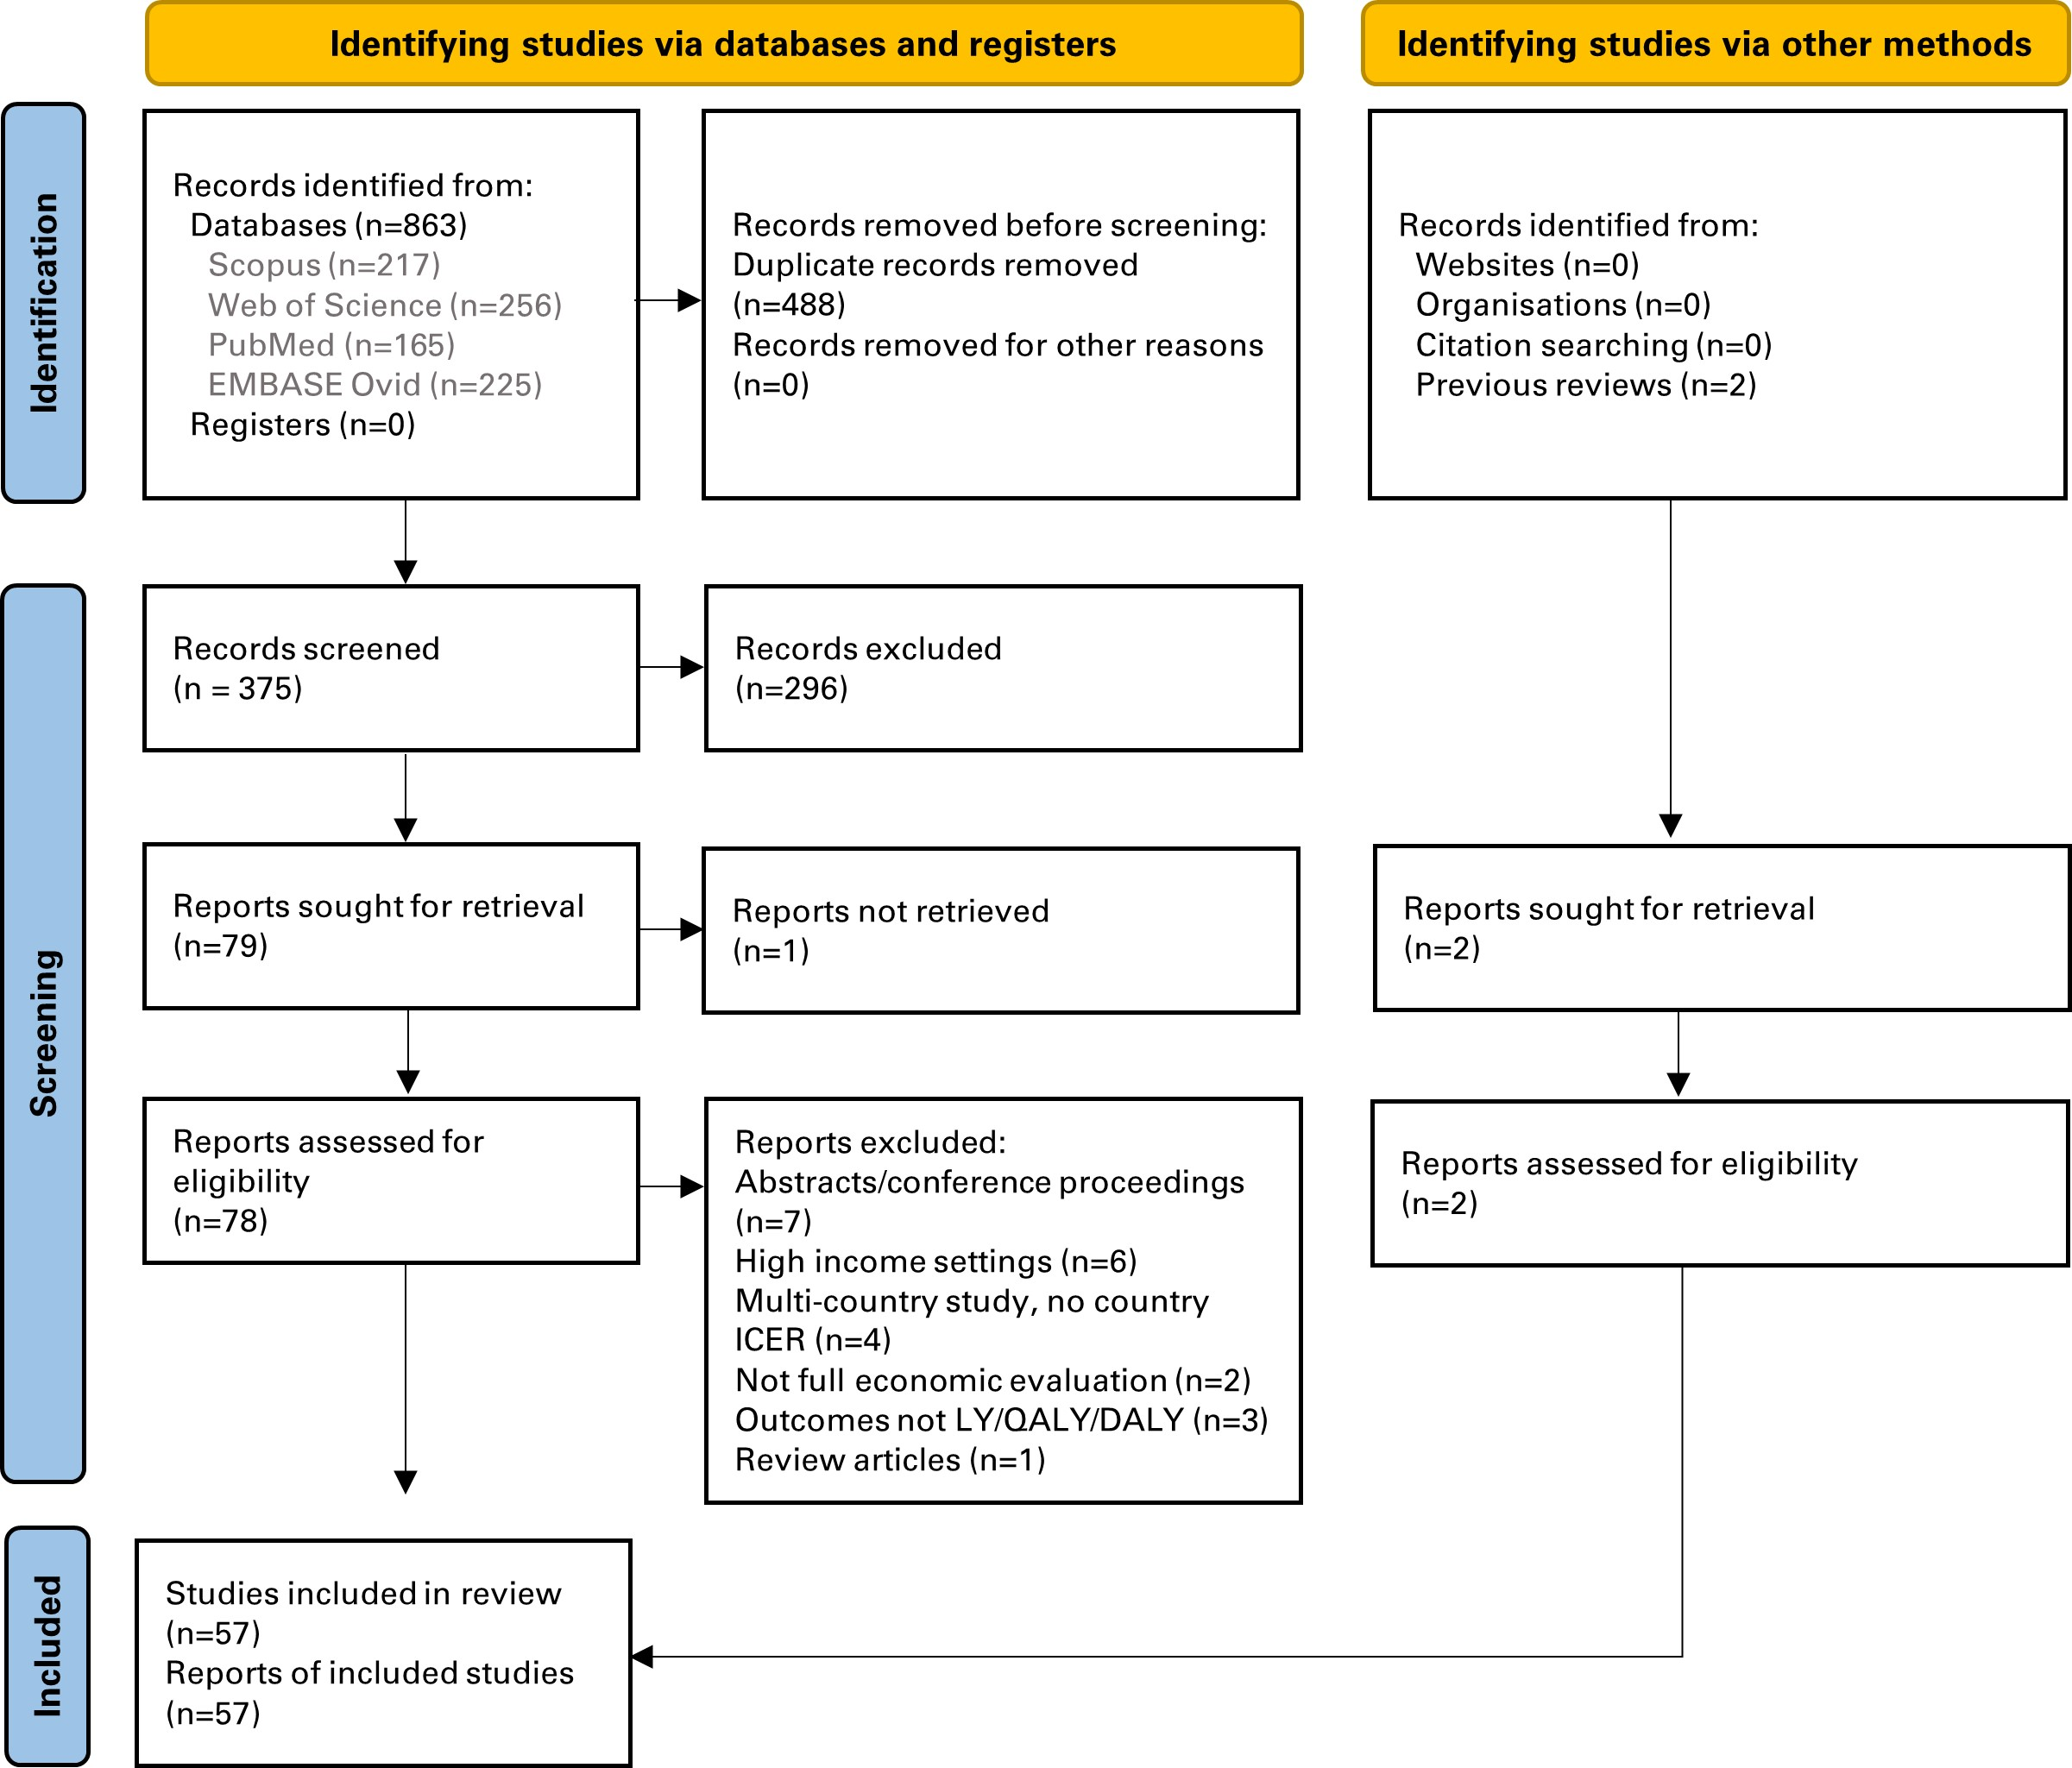
\includegraphics[width=1\linewidth]{figures/prisma-flow-diagram.jpg}
    \caption{PRISMA flow diagram.}
    \label{fig:prisma-flow-diagram}
    \caption*{\footnotesize \textit{}}
\end{figure}

\subsection{Factors associated with switching from cost-effective to not cost-effective}
[In progress]
Descriptively, evaluations that switched from being cost-effective to not cost-effective under any of the updated CETs were more likely to be comparisons between PCV7 versus no vaccination or PCV10 versus no vaccination. They were also more likely to be conducted in lower income settings, not to consider herd immunity, but to consider serotype replacement . None of these associations were statistically significant according to the Pearson Chi squared test. No relationship was found between perspective of analysis and the evaluation switching from begin cost-effective. However, evaluations that switched from being cost-effective to not cost-effective across any of the new CETs had statistically higher mean vaccine dose price: \$27.7  vs \$15.5 (mean difference \$12.2, 95\% confidence interval, 2.9 to 21.4). 

Probit regression results found vaccine dose price and country income group were the only statistically significant variables related to evaluations switching from being cost-effective to not cost-effective across any one of the updated CETs.




\begin{table}[H]
    \centering \singlespacing \small
    \caption{Likelihood of switching}
    \begin{tabular}{|L{4.5cm}|L{4cm}|C{2.75cm}|C{2.75cm}|}
        \hline
        \PlainInput{tables/tab_likely_anyswitch}
    \end{tabular}
    \label{tab_likely_anyswitch}
    \caption*{\footnotesize \textit{Notes:} Other evaluations included PCV9 vs NoVax, PCV13 vs PCV7, and PCV10 vs PCV7. \\
    IPD, invasive pneumococcal disease; PCV, pneumococcal conjugate vaccine; PCV7, 7-valent PCV; PCV10, 10-valent PCV; PCV13, 13-valent PCV. 
}
\end{table}


\subsection{Sensitivity analyses}
[In progress]


\section{Discussion}
\subsection{Interpretation of results}
[In progress]

\subsection{Strengths and limitation}
Multi-country studies.66-69 why don't they report at country-level – this would be useful !
[In progress by Natalie]
Strength: first paper to our knowledge to consider the impact of new, lower CETs on conclusions of cost-effectiveness across LMICs
Limitation: only considering base case ICERs, and ICERs available by differing perspective (health care payer vs societal), and with or without herd effects and/or serotype replacement.
Do not include all ICERs reported by studies (ex: through sensitivity or scenario analyses exploring different vaccine dose prices etc)

Compare results with countries that have or have not introduced PCV. Goal is not to suggest PCV should not be introduced or should be removed if not CE . But introducing a technology/vaccine when ICER exceeds WTP could be detrimental – money could be better spent on other things .
Goal – to revisit cost-effectiveness and understand whether further price negotiations are necessary . Examples of price negotiations from other settings (Indonesia? Thailand?? Ask Sarin and Itob). 

To do later:
Among low-income countries, xYZ 
Among middle-income countries – what trends do we see and does that vary by vaccine price and/or taking herd effects into account?
-	CETs are likely to vary over time, which has not been considered here
-	Further analyses to look at associations between shifts in decision-making and characteristics of evaluations.
-	Further work could link these evaluations to actual policy decisions in countries to introduce PCV (or not)
Implications for PCV Policy
[In progress]


%%%%%%%%%%%%%%%%%%%%%%%%%%%%
%%% %%%
%%% Bibliography %%%

\clearpage
\printbibliography


\end{document}
